%
% einleitung.tex -- Beispiel-File für die Einleitung
%
% (c) 2020 Prof Dr Andreas Müller, Hochschule Rapperswil
%
% !TEX root = ../../buch.tex
% !TEX encoding = UTF-8
%
\subsection{Zylinder\label{geodaeten:section:Standardverfahren:Zylinder}}
\rhead{Standardverfahren Beispiele}

Für die Zylinder Oberfläche mit konstantem $r$, mit dem metrischen Tensor 
\begin{equation}
	g_{ij} = \begin{pmatrix} 
		r^2 & 0 \\ 
		0 & 1 
	\end{pmatrix},
\end{equation}

wollen wir die Christophsymbole berechnen. 
Wie bei dem kartesischen Raum (Abschnitt \ref{geodaeten:section:Standardverfahren:Kartesisch}) werden alle Christophsymbole Null, da der metrische Tensor konstant ist.\footnote{
Auch in diesem Beispiel sind die Christophsymbole gleich Null.
Auf den ersten Blick könnte das verwirrend sein, da man bei einem Zylinder doch eindeutig eine Krümmung sieht.
Der Grund dafür ist, dass es sich bei dem Zylinder um eine extrinsische Krümmung handelt.
Die Zylinderoberfläche wird von außen zu einem Zylinder gekrümmt.
Abgerollt sieht man allerdings, dass die Oberfläche Flach ist.
Als weiteres Beispiel lässt sich berechnen, dass die Christophsymbole im Polarkoordinaten-Raum nicht gleich Null sind und daher eine Krümmung existiert, obwohl der Raum Flach erscheint.
Damit zeigt sich, dass die Intuition in diesem Fall täuschen kann.
}
Wir ersparen uns hier deshalb diese Rechnung.

Setzt man so $u^1 = \phi (t)$ und $u^2 = z(t)$ in die Geodätengleichung ein, so erhält man analog zu [\ref{geodaeten:equation:Standardverfahren:Kartesisch:x}]
\begin{equation}
	\ddot{\phi}(t) = 0
	\label{geodaeten:equation:Standardverfahren:Zylinder:phi}
\end{equation}

und dementsprechend gemäß [\ref{geodaeten:equation:Standardverfahren:Kartesisch:y}] 
\begin{equation}
	\ddot{z}(t) = 0 .
\end{equation}

Wählen wir $P_A(\phi_1 , z_1) = P_A(1 , 1)$ und $P_B(\phi_2 , z_2) = P_B(3 , 5)$ gleich wie in Abschnitt \ref{geodaeten:section:Standardverfahren:Kartesisch}, kennen wie bereits die Lösungen

\begin{equation}
	\phi(t) = 2t + 1 .
\end{equation}

\begin{equation}
	z(t) = 4t + 1 .
\end{equation}

Beim Zylinder ist jedoch interessant, dass es beliebige Lösungen für die Geodätengleichung gibt, da Die Winkelkoordinate Periodisch ist.
Durch Hinzufügen eines vielfachen von $2\pi$ macht die Kurve zusätzliche Runden um den Zylinder bevor es auf den Punkt $P_B$ trifft.
Dies ist zwar nicht die kürzeste Strecke, jedoch weder die Gleichung \ref{geodaeten:equation:Standardverfahren:Zylinder:phi} verletz noch der Punkt $P_a$ oder $P_B$ verfehlt.
Deshalb existieren sie als Scheinlösungen der Geodätengleichung.

Auch interessant ist, dass wenn die Oberfläche des Zylinders abgerollt auf eine Fläche dargestellt wird, ersichtlich ist, wie auch hier der kürzeste Weg eine Gerade ist.  

\begin{figure}
	\centering
	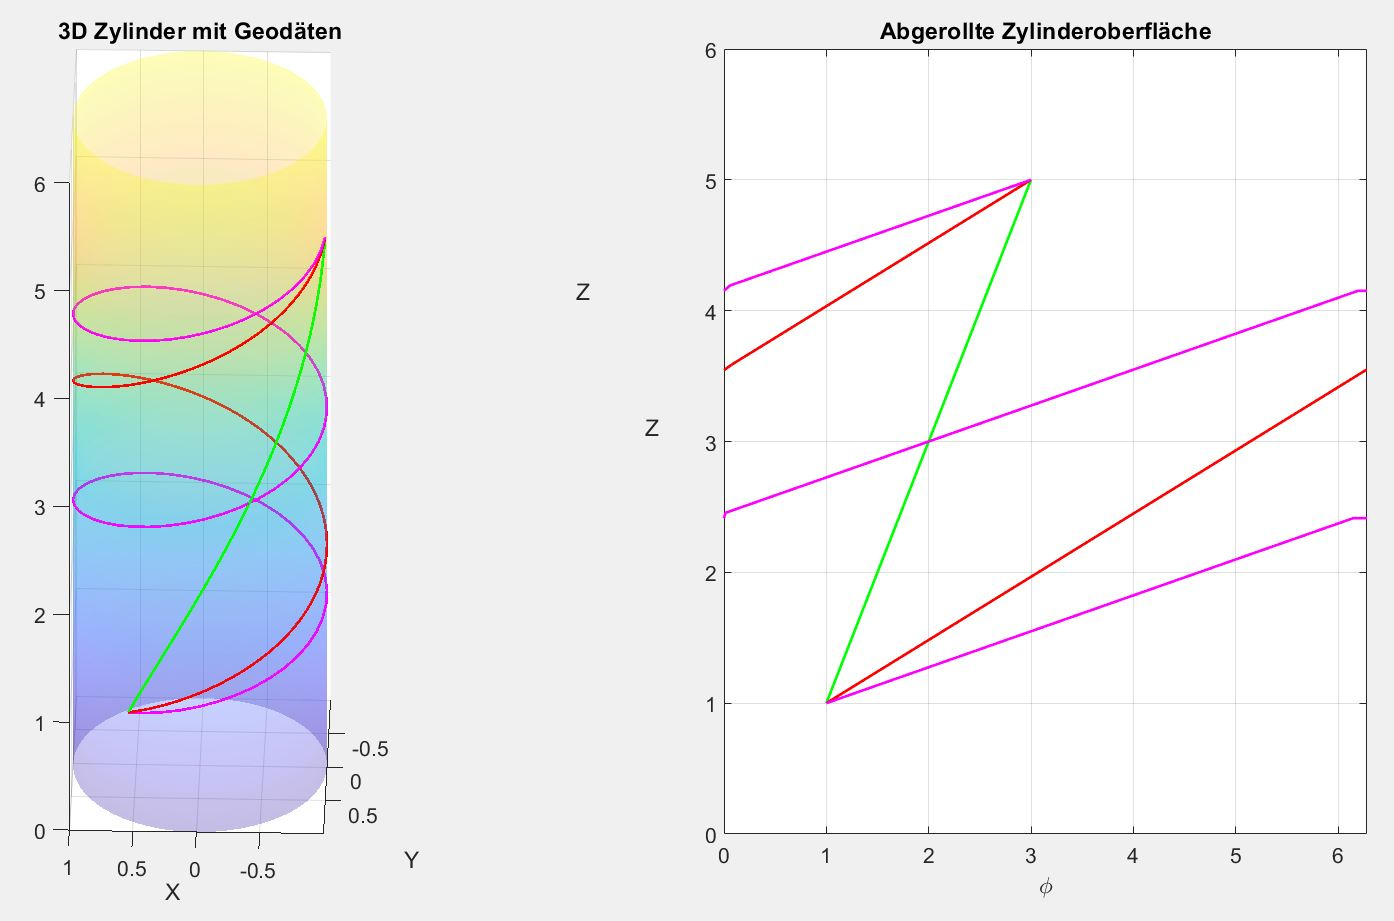
\includegraphics[width=14cm]{papers/geodaeten/Abbildungen/Standardverfahren/Zylinder}
	\caption{Darstellung der Geodätenlinien auf einem Zylinder und dessen abgerollte Oberfläche in einem 2D Plot mit Matlab}
	\label{geodaeten:figure:Linienelemente:Zylinder:figure1}
\end{figure}
